\documentclass{beamer}
\usetheme{Madrid}
\setbeamertemplate{bibliography item}{\insertbiblabel}

\usepackage[main=english,czech]{babel}
\usepackage[utf8]{inputenc}
\usepackage{url}
\usepackage{caption}

\captionsetup[figure]{font=footnotesize}

%\usepackage{biblatex}
%\addbibresource{references.bib}

\AtBeginSection[]
{
	\begin{frame}<beamer>[noframenumbering]
		\frametitle{Outline}
		\tableofcontents[currentsection]
	\end{frame}
}

\title[Runge-Kutta Algorithm Energy Resolution]{Energy Resolution of Runge-Kutta Reconstruction of Padded Microscopically Simulated Tracks}
\subtitle{First Successful Attempt}
\author[M.~Vavřík]{\foreignlanguage{czech}{Martin Vavřík}\vspace{0.5cm}\\martin.vavrik@cvut.cz\\IEAP CTU PRAGUE\\}
\logo{
\includegraphics[width=0.08\textwidth]{images/logo}}
\date{November 10, 2023}

\begin{document}
	
	\begin{frame}
		\titlepage
	\end{frame}
	
	\begin{frame}
		\frametitle{Outline}
		\tableofcontents
	\end{frame}
	
	\section{Grid-like track simulation}
		\begin{frame}
			\frametitle{Grid-like track simulation}
			\begin{itemize}
				\item We use Garfield++ for track simulation
				\begin{itemize}
					\item Primary relativistic particle simulated using Heed program~\cite{heed}
					\item Secondary ionization electrons simulated using microscopic tracking (uses equation of motion)
				\end{itemize}
				\item Microscopic tracks were simulated on MetaCentrum to test the Runge-Kutta padded reconstruction
				\begin{itemize}
					\item 2000 jobs, each 20-160 hours runtime, 20~GB RAM allocated
					\item 9702 tracks were simulated (electron vs positron, 21~theta angles, 21~phi angles, 11~energies 3-13~MeV)
					\item Reconstruction lasts around 40~minutes
				\end{itemize}
			\end{itemize}
		\end{frame}
		
		\begin{frame}
		\frametitle{Simulation ranges}
			\begin{figure}
				\centering
				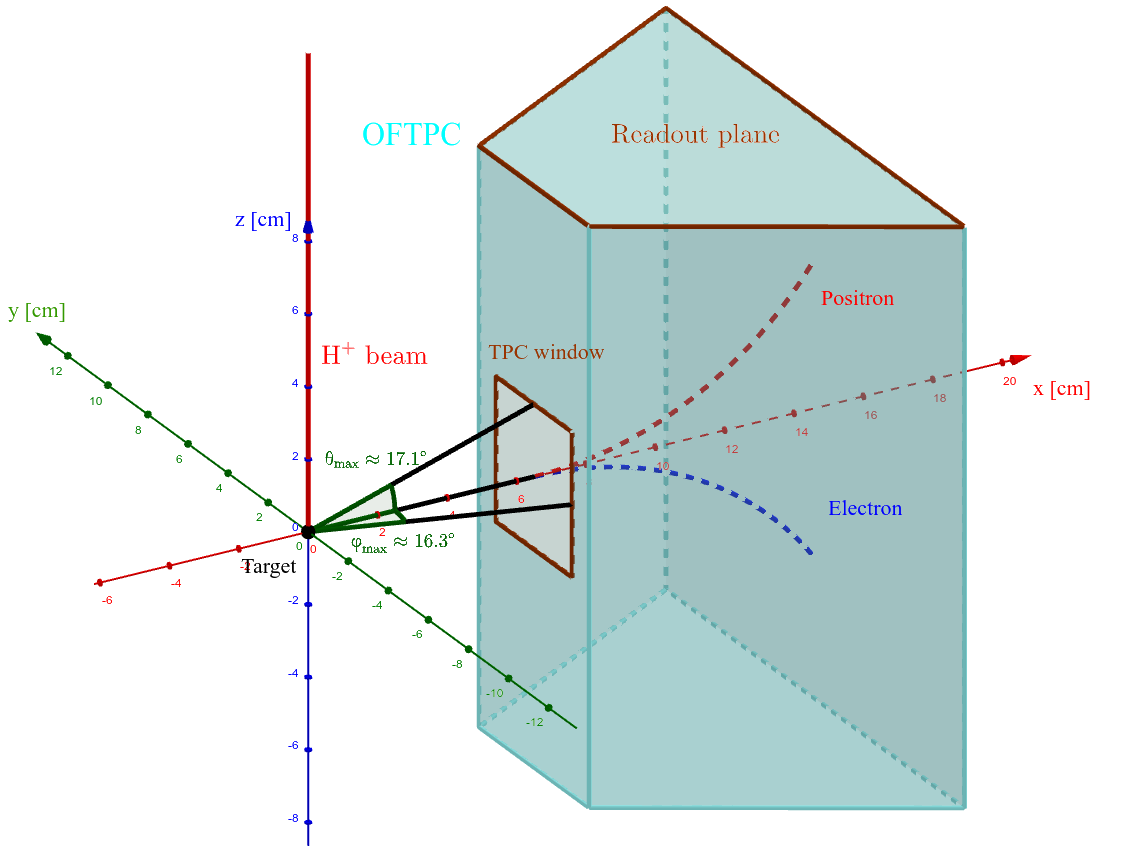
\includegraphics[width = 0.9 \linewidth]{images/tpc_micro_simulation.png}
				\caption{$\theta \in [-17.1^\circ,17.1^\circ]$, $\varphi \in [-16.3^\circ,16.3^\circ]$, $ E_k \in [3,13] $~MeV.}
			\end{figure}
		\end{frame}
	
	\section{Direction independent resolution}
	
		\begin{frame}
			\frametitle{Energy resolution for all tracks}
			\begin{columns}
				\column{0.5\textwidth}
				\centering
				\Large \textbf{Electrons}
				\begin{figure}
					\centering
					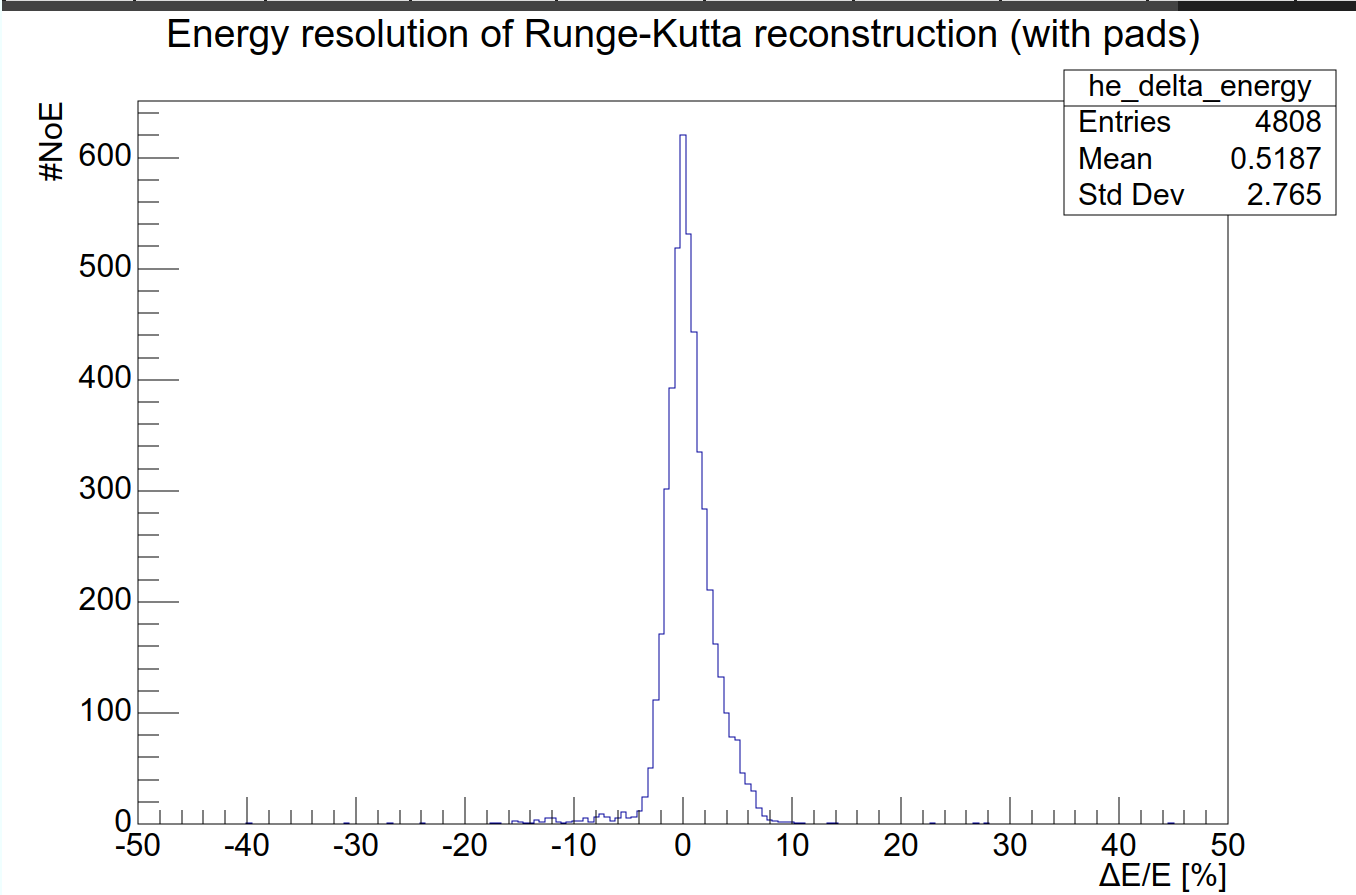
\includegraphics[width = 0.95 \linewidth]{images/c_e_delta_energy.png}
				\end{figure}
				\column{0.5\textwidth}
				\centering
				\Large \textbf{Positrons}
				\begin{figure}
					\centering
					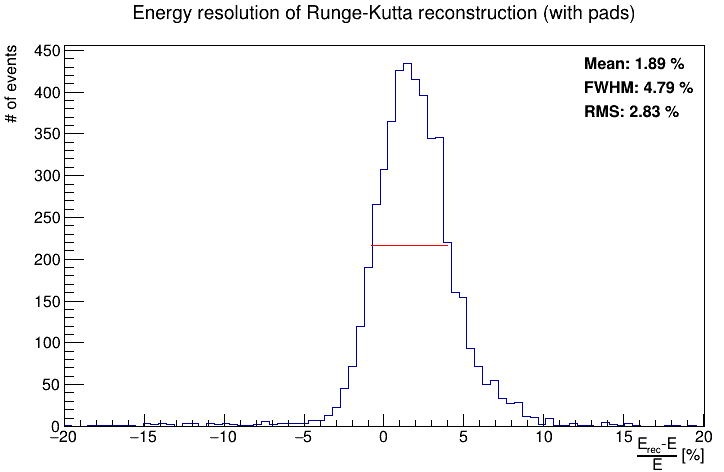
\includegraphics[width = 0.95 \linewidth]{images/c_p_delta_energy.png}
				\end{figure}
			\end{columns}
		\end{frame}
		\begin{frame}
			\frametitle{Energy resolution dependence on simulated energy}
			\begin{columns}
				\column{0.5\textwidth}
				\centering
				\Large \textbf{Electrons}
				\begin{figure}
					\centering
					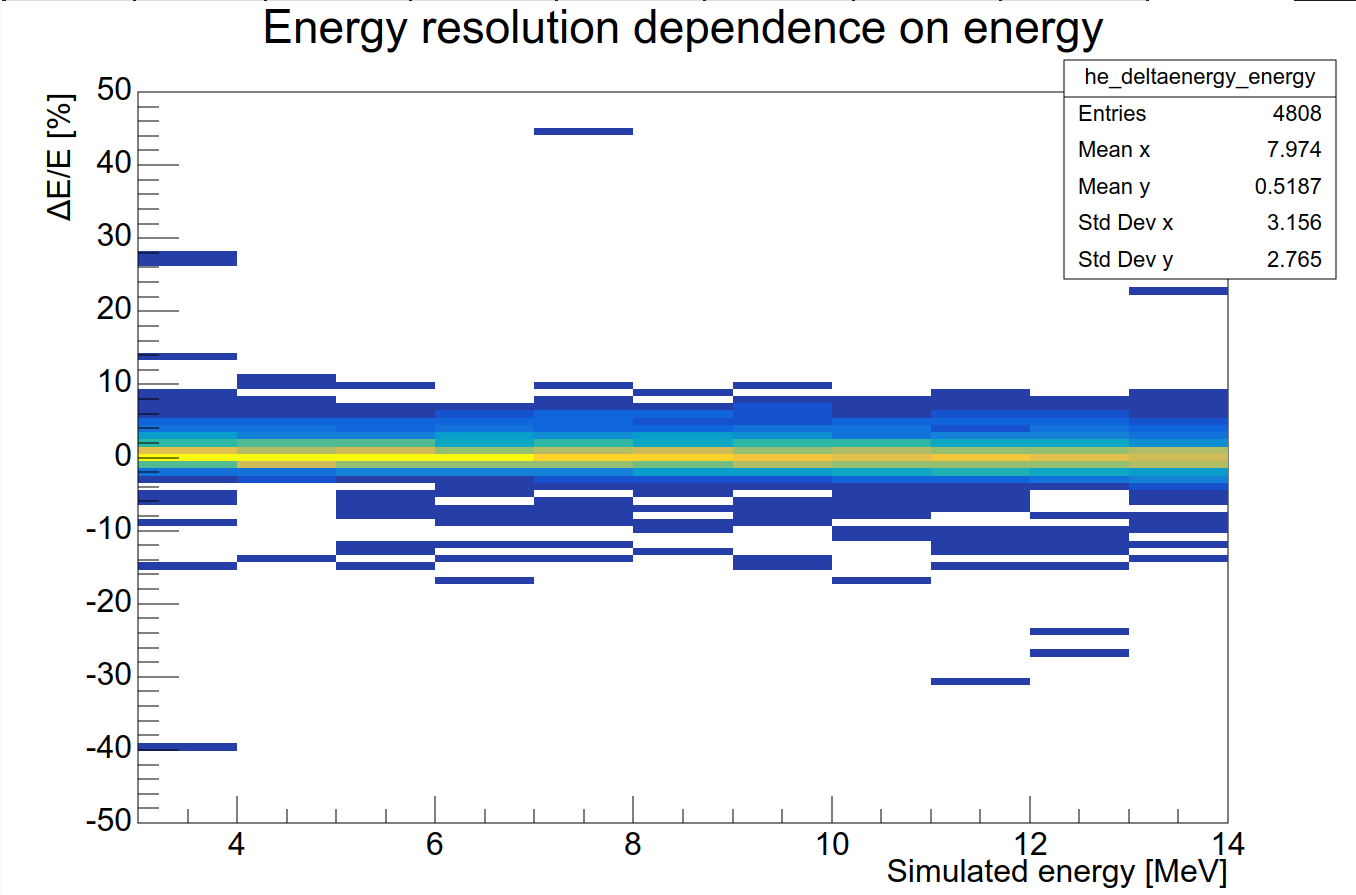
\includegraphics[width = 0.95 \linewidth]{images/c_e_deltaenergy_energy.png}
				\end{figure}
				\column{0.5\textwidth}
				\centering
				\Large \textbf{Positrons}
				\begin{figure}
					\centering
					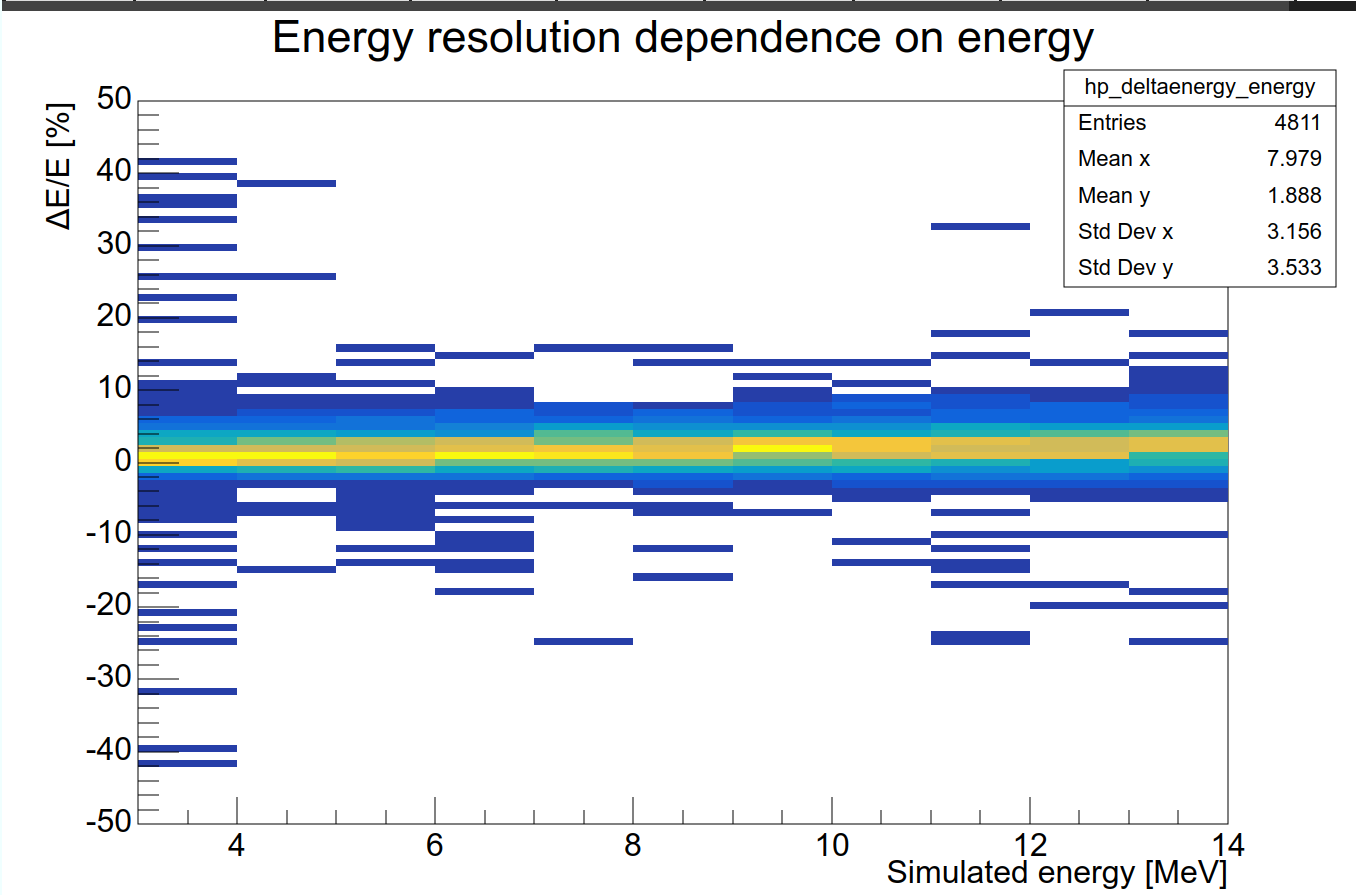
\includegraphics[width = 0.95 \linewidth]{images/c_p_deltaenergy_energy.png}
				\end{figure}
			\end{columns}
		\end{frame}
		
	\section{Direction dependent resolution}
	
		\begin{frame}
			\frametitle{Energy resolution dependence on phi}
			\begin{columns}
				\column{0.5\textwidth}
				\centering
				\Large \textbf{Electrons}
				\begin{figure}
					\centering
					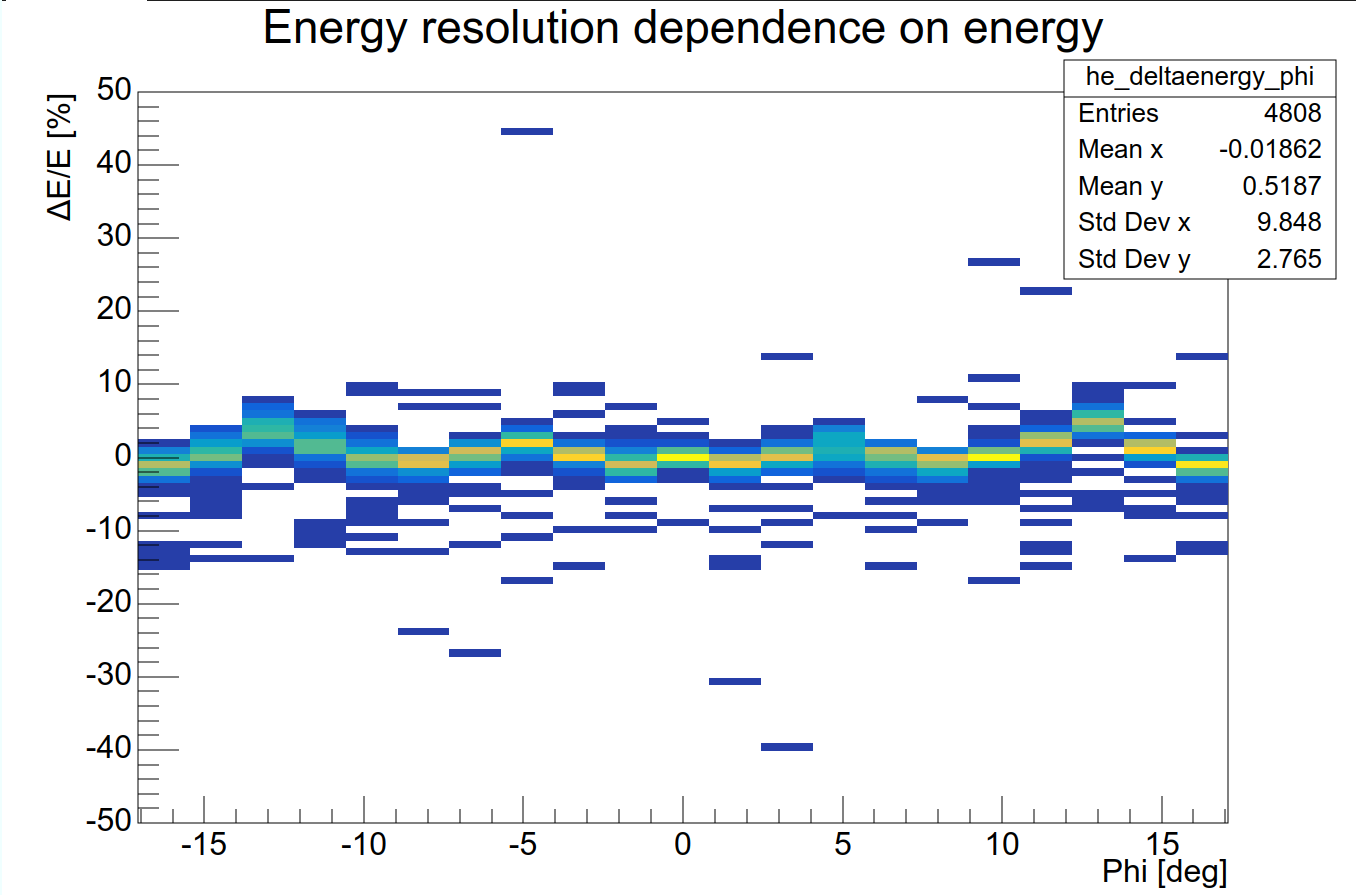
\includegraphics[width = 0.95 \linewidth]{images/c_e_deltaenergy_phi.png}
				\end{figure}
				\column{0.5\textwidth}
				\centering
				\Large \textbf{Positrons}
				\begin{figure}
					\centering
					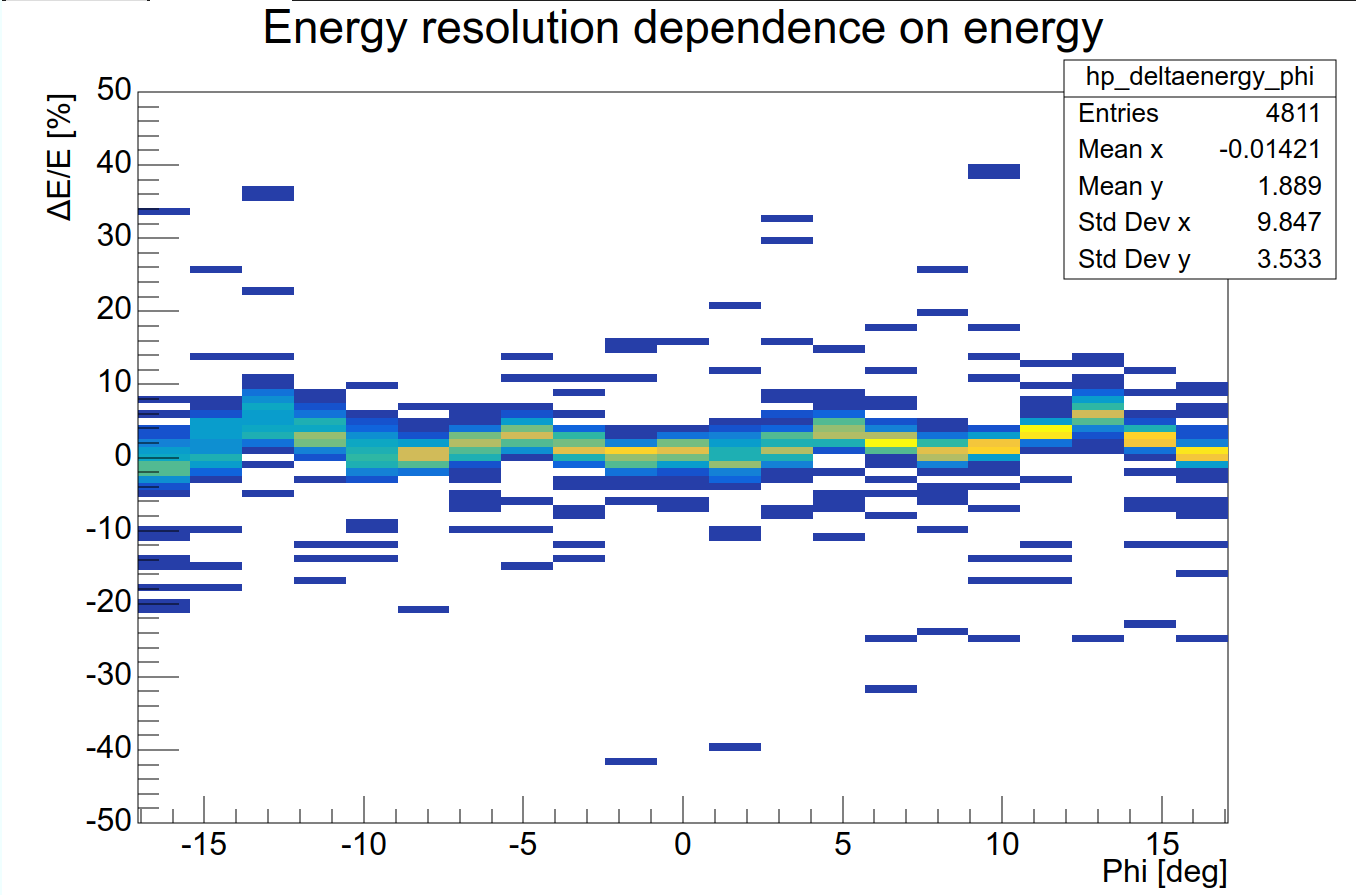
\includegraphics[width = 0.95 \linewidth]{images/c_p_deltaenergy_phi.png}
				\end{figure}
			\end{columns}
		\end{frame}
		\begin{frame}
			\frametitle{Energy resolution dependence on theta}
			\begin{columns}
				\column{0.5\textwidth}
				\centering
				\Large \textbf{Electrons}
				\begin{figure}
					\centering
					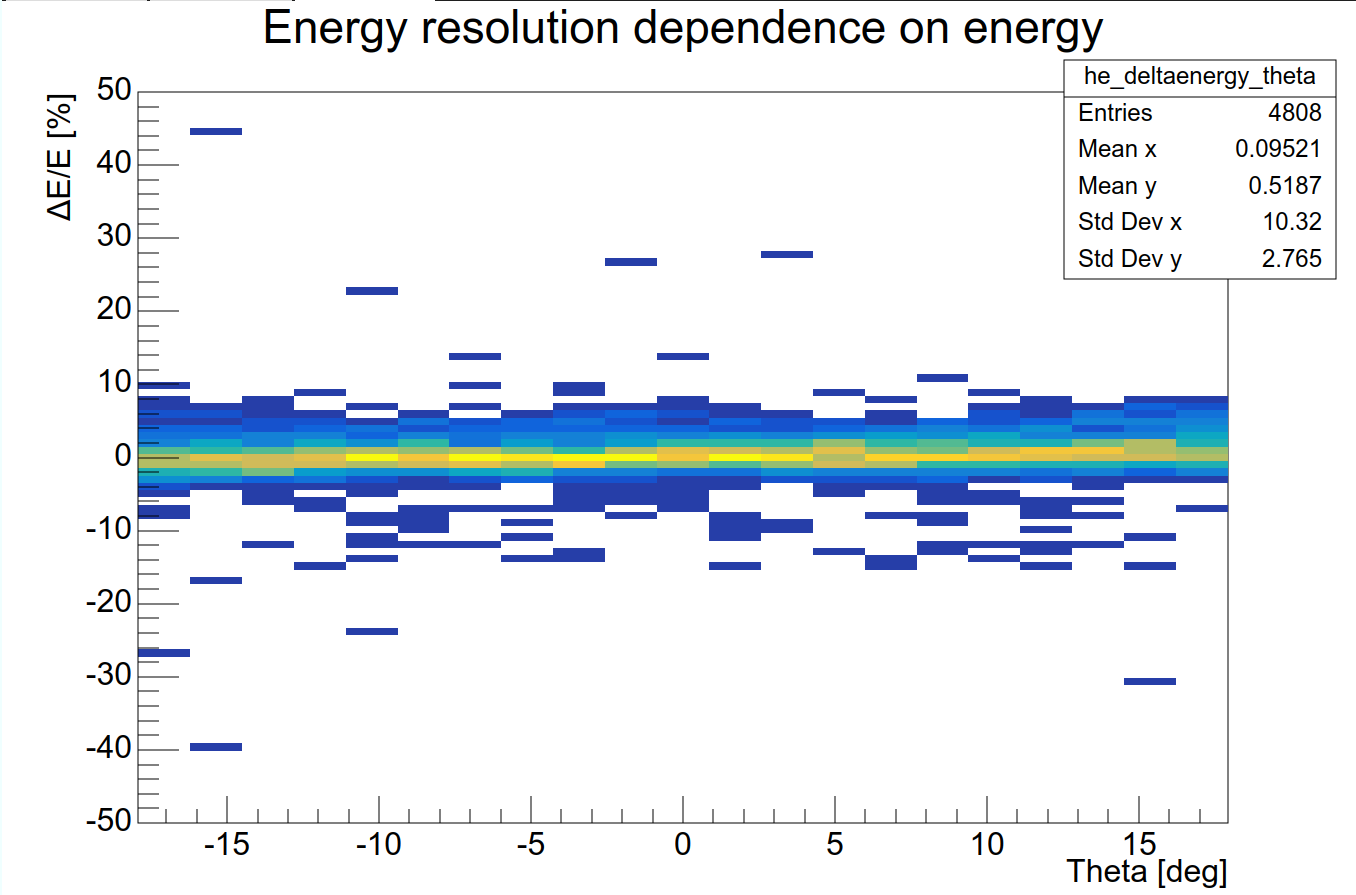
\includegraphics[width = 0.95 \linewidth]{images/c_e_deltaenergy_theta.png}
				\end{figure}
				\column{0.5\textwidth}
				\centering
				\Large \textbf{Positrons}
				\begin{figure}
					\centering
					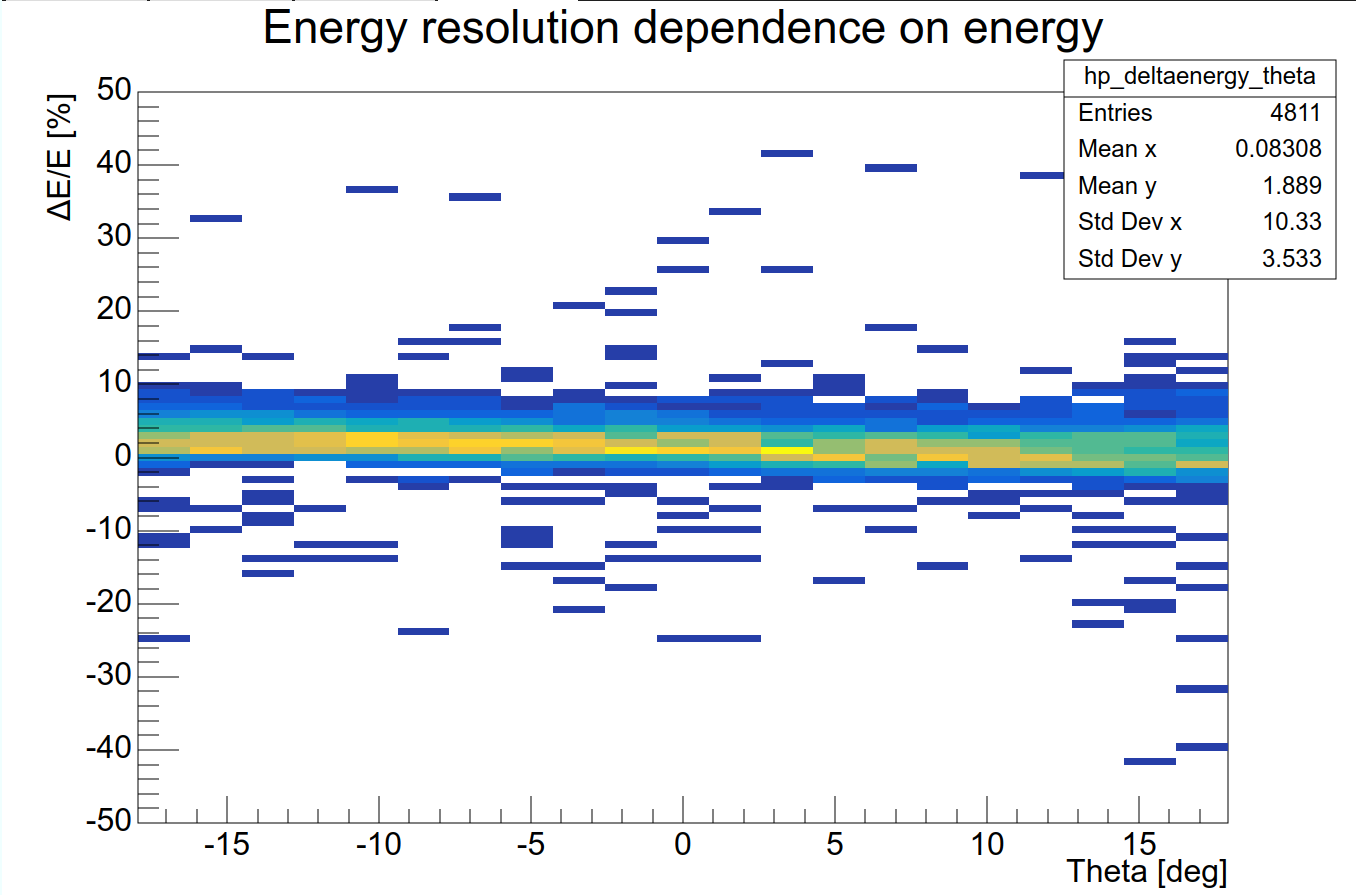
\includegraphics[width = 0.95 \linewidth]{images/c_p_deltaenergy_theta.png}
				\end{figure}
			\end{columns}
		\end{frame}
	
	\section{All track parameters dependence}
	
	\begin{frame}
		\frametitle{All track parameters (phi, theta and simulated energy)}		
		\begin{columns}
			\column{0.5\textwidth}
			\centering
			\Large \textbf{Electrons}
			\begin{figure}
				\centering
				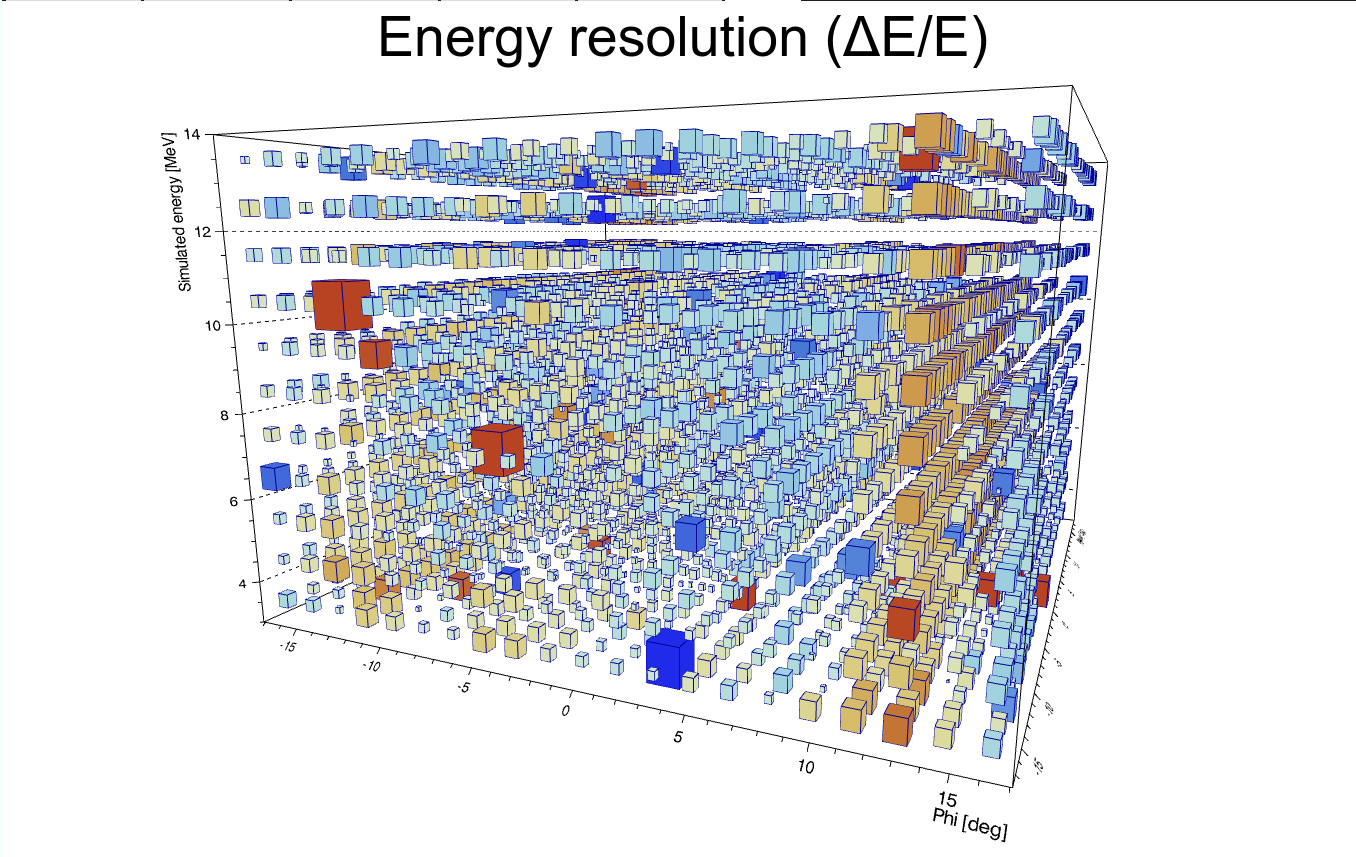
\includegraphics[width = 0.95 \linewidth]{images/c_e_all.png}
			\end{figure}
			\column{0.5\textwidth}
			\centering
			\Large \textbf{Positrons}
			\begin{figure}
				\centering
				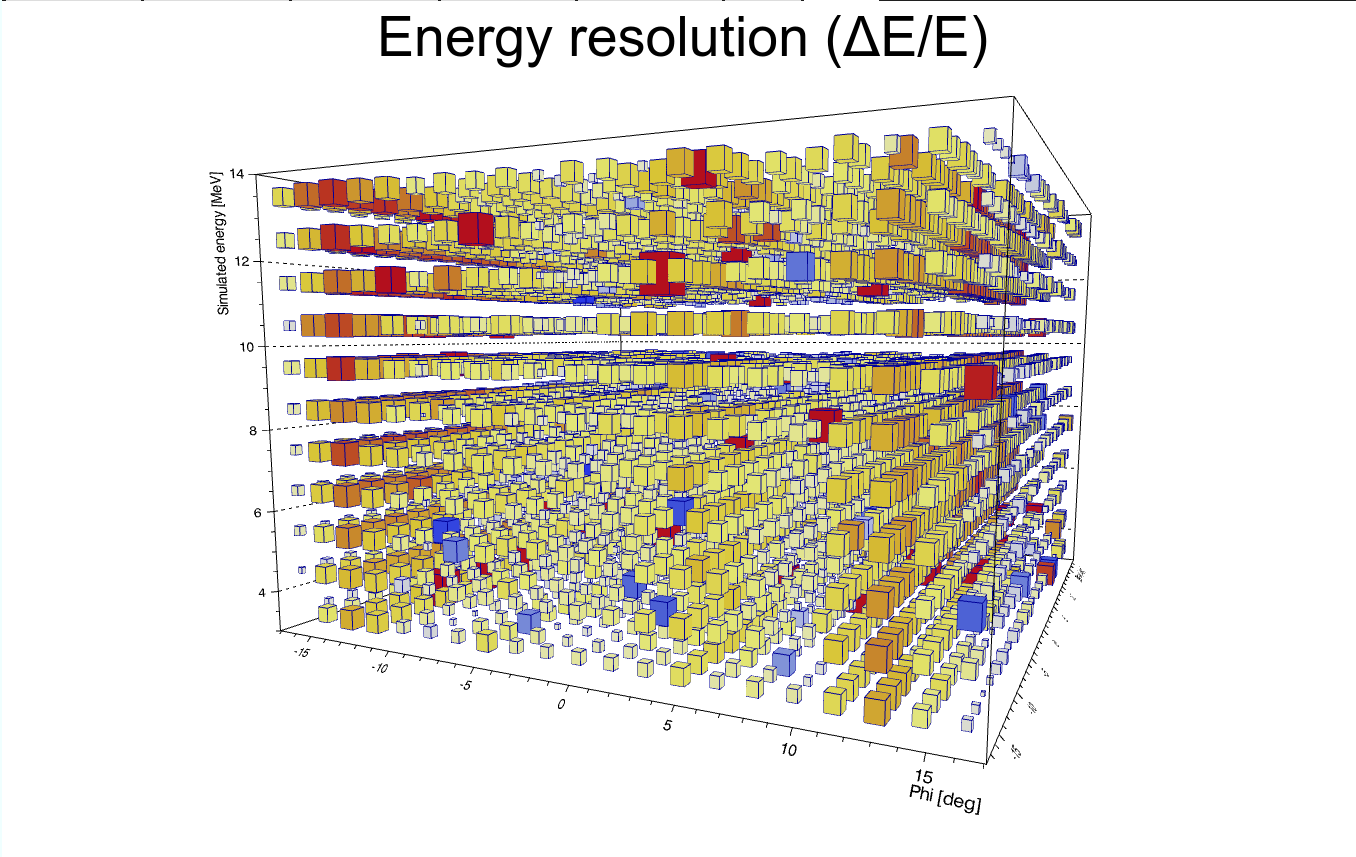
\includegraphics[width = 0.95 \linewidth]{images/c_p_all.png}
			\end{figure}
		\end{columns}
	\end{frame}
	
	
	\section{2D cuts average bias}
	
		\begin{frame}
			\frametitle{Theta-Phi cut average bias}
			\begin{columns}
				\column{0.5\textwidth}
				\centering
				\Large \textbf{Electrons}
				\begin{figure}
					\centering
					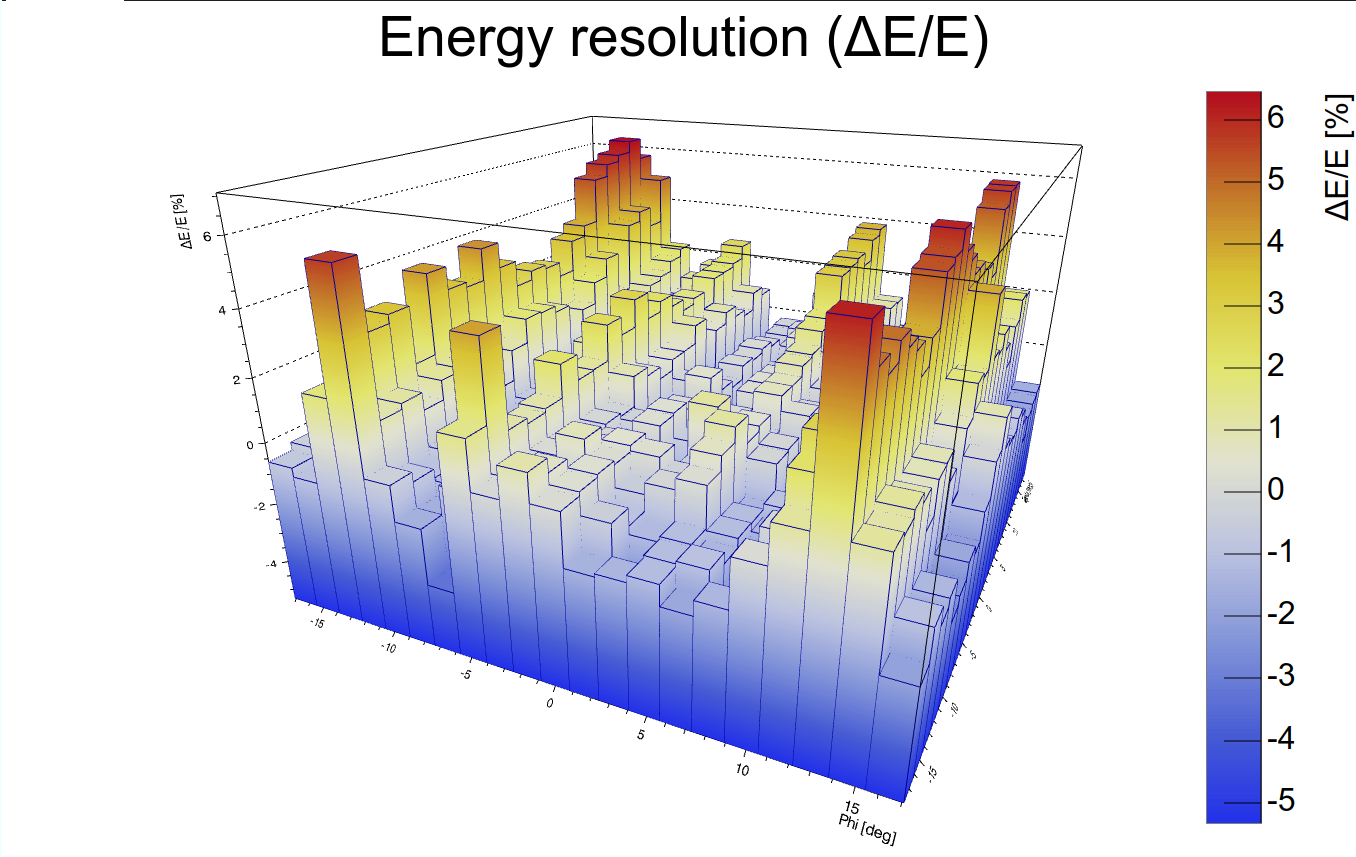
\includegraphics[width = 0.95 \linewidth]{images/c_e_theta_phi.png}
				\end{figure}
				\column{0.5\textwidth}
				\centering
				\Large \textbf{Positrons}
				\begin{figure}
					\centering
					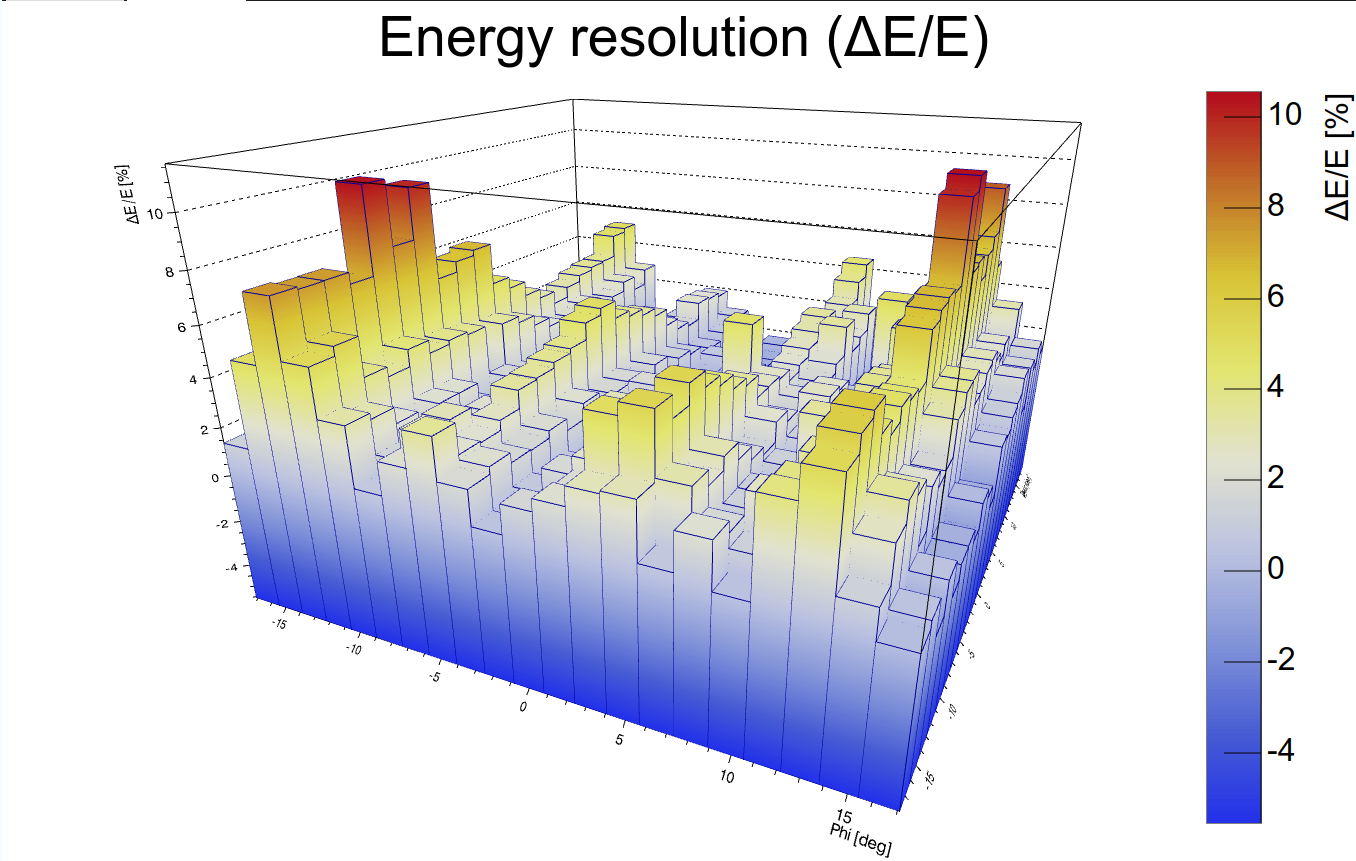
\includegraphics[width = 0.95 \linewidth]{images/c_p_theta_phi.png}
				\end{figure}
			\end{columns}
		\end{frame}
		\begin{frame}
			\frametitle{Theta-Energy cut average bias}
			\begin{columns}
				\column{0.5\textwidth}
				\centering
				\Large \textbf{Electrons}
				\begin{figure}
					\centering
					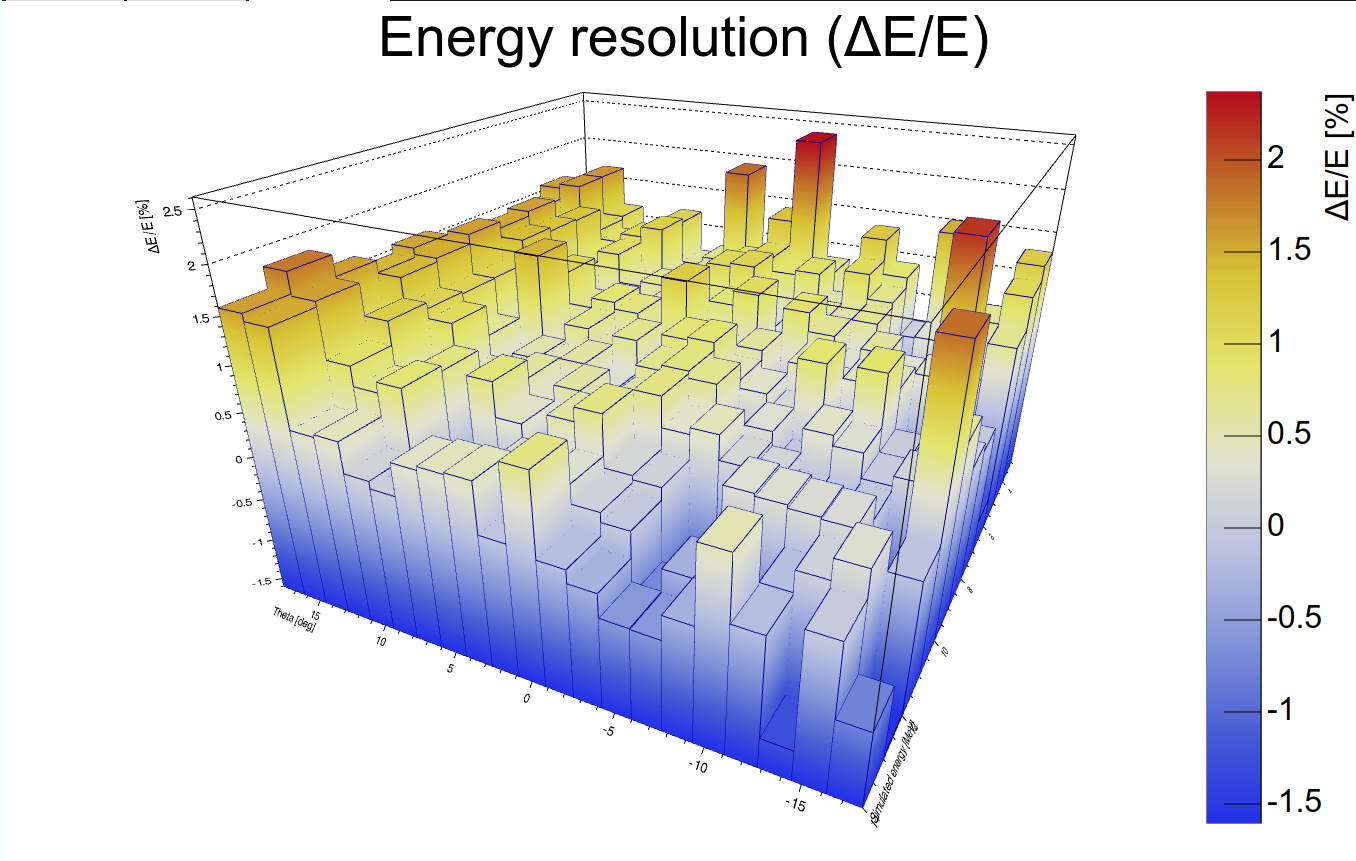
\includegraphics[width = 0.95 \linewidth]{images/c_e_theta_energy.png}
				\end{figure}
				\column{0.5\textwidth}
				\centering
				\Large \textbf{Positrons}
				\begin{figure}
					\centering
					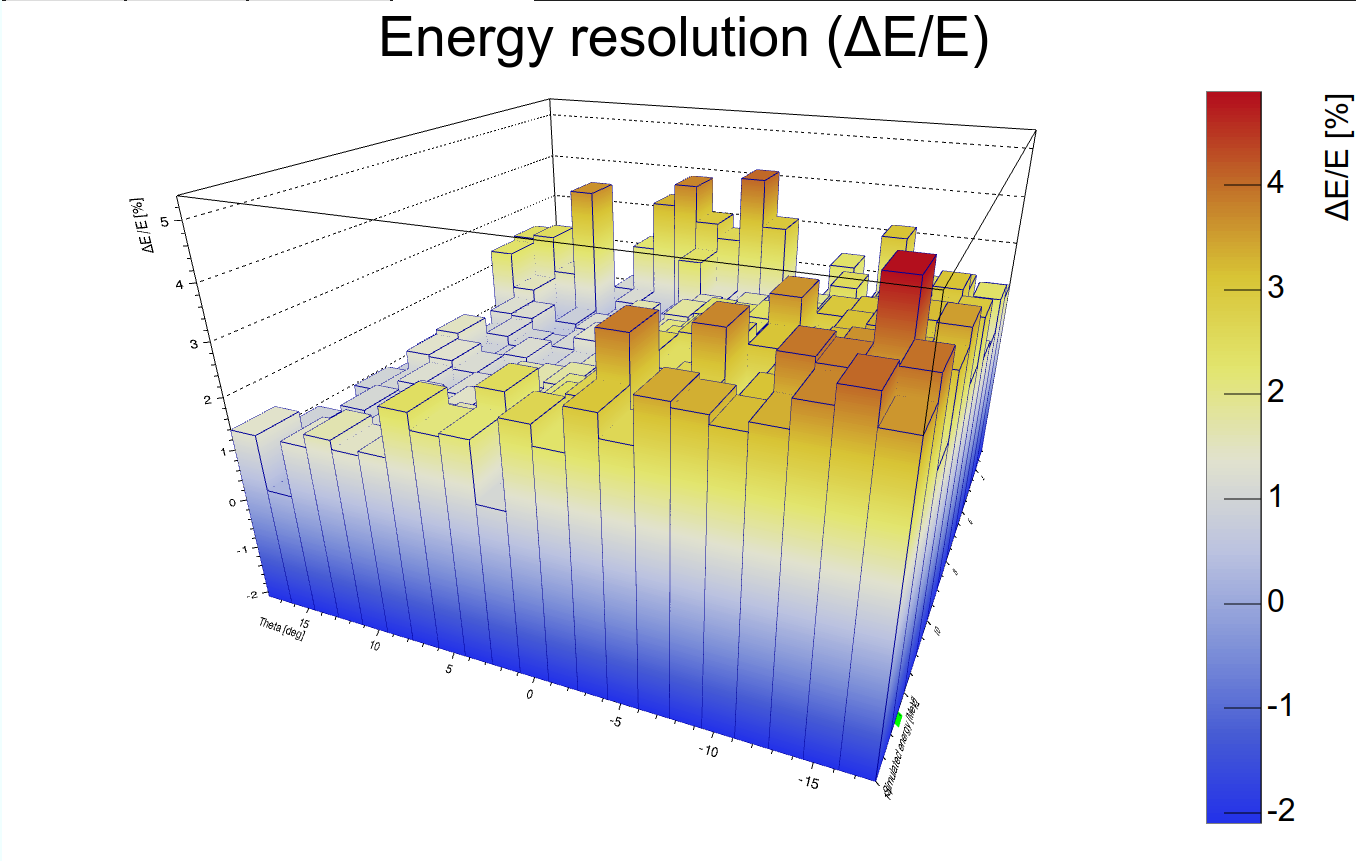
\includegraphics[width = 0.95 \linewidth]{images/c_p_theta_energy.png}
				\end{figure}
			\end{columns}
		\end{frame}
		\begin{frame}
			\frametitle{Phi-Energy cut average bias}
			\begin{columns}
				\column{0.5\textwidth}
				\centering
				\Large \textbf{Electrons}
				\begin{figure}
					\centering
					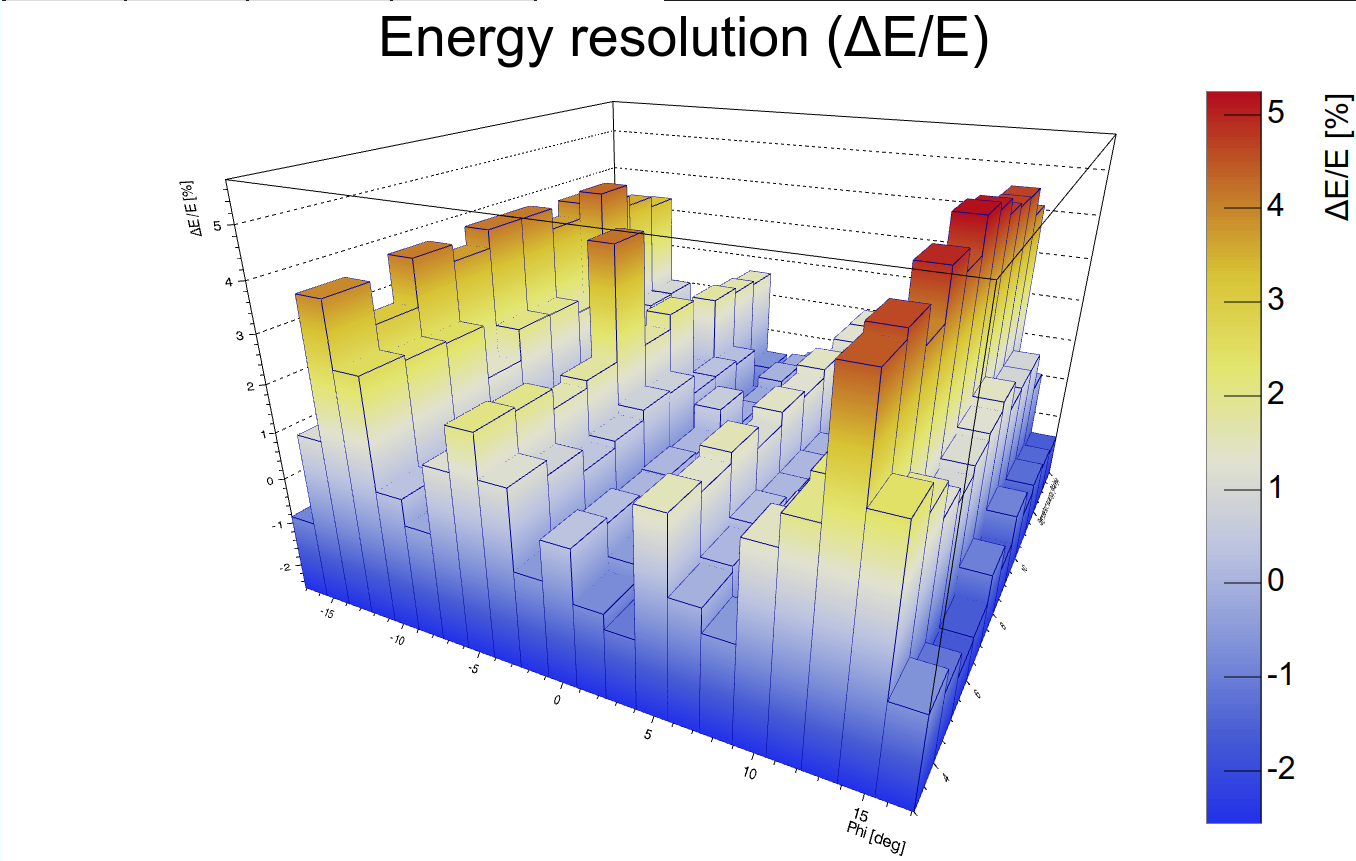
\includegraphics[width = 0.95 \linewidth]{images/c_e_phi_energy.png}
				\end{figure}
				\column{0.5\textwidth}
				\centering
				\Large \textbf{Positrons}
				\begin{figure}
					\centering
					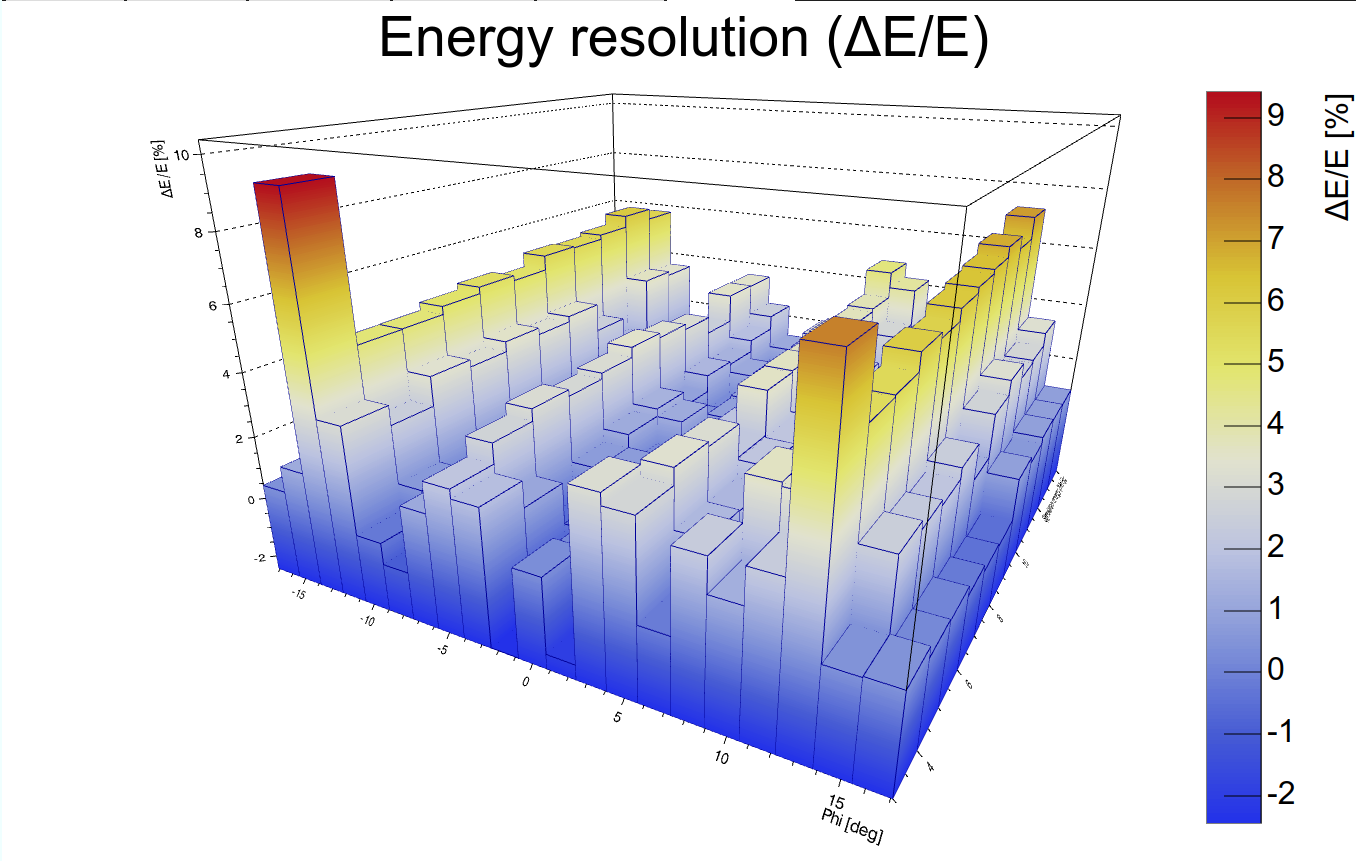
\includegraphics[width = 0.95 \linewidth]{images/c_p_phi_energy.png}
				\end{figure}
			\end{columns}
		\end{frame}
	
	\section{2D cuts average error}
	
		\begin{frame}
			\frametitle{Theta-Phi cut average error}
			\begin{columns}
				\column{0.5\textwidth}
				\centering
				\Large \textbf{Electrons}
				\begin{figure}
					\centering
					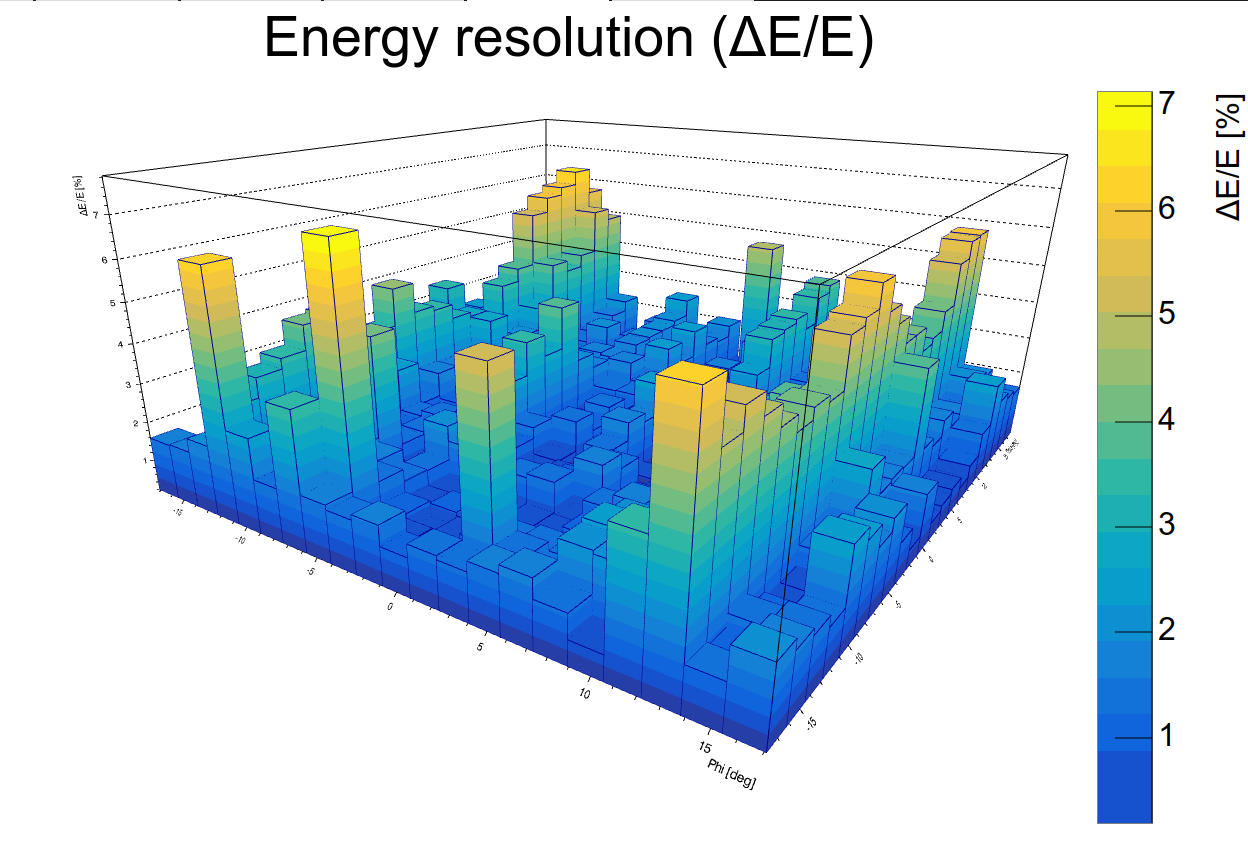
\includegraphics[width = 0.95 \linewidth]{images/c_e_theta_phi_abs.png}
				\end{figure}
				\column{0.5\textwidth}
				\centering
				\Large \textbf{Positrons}
				\begin{figure}
					\centering
					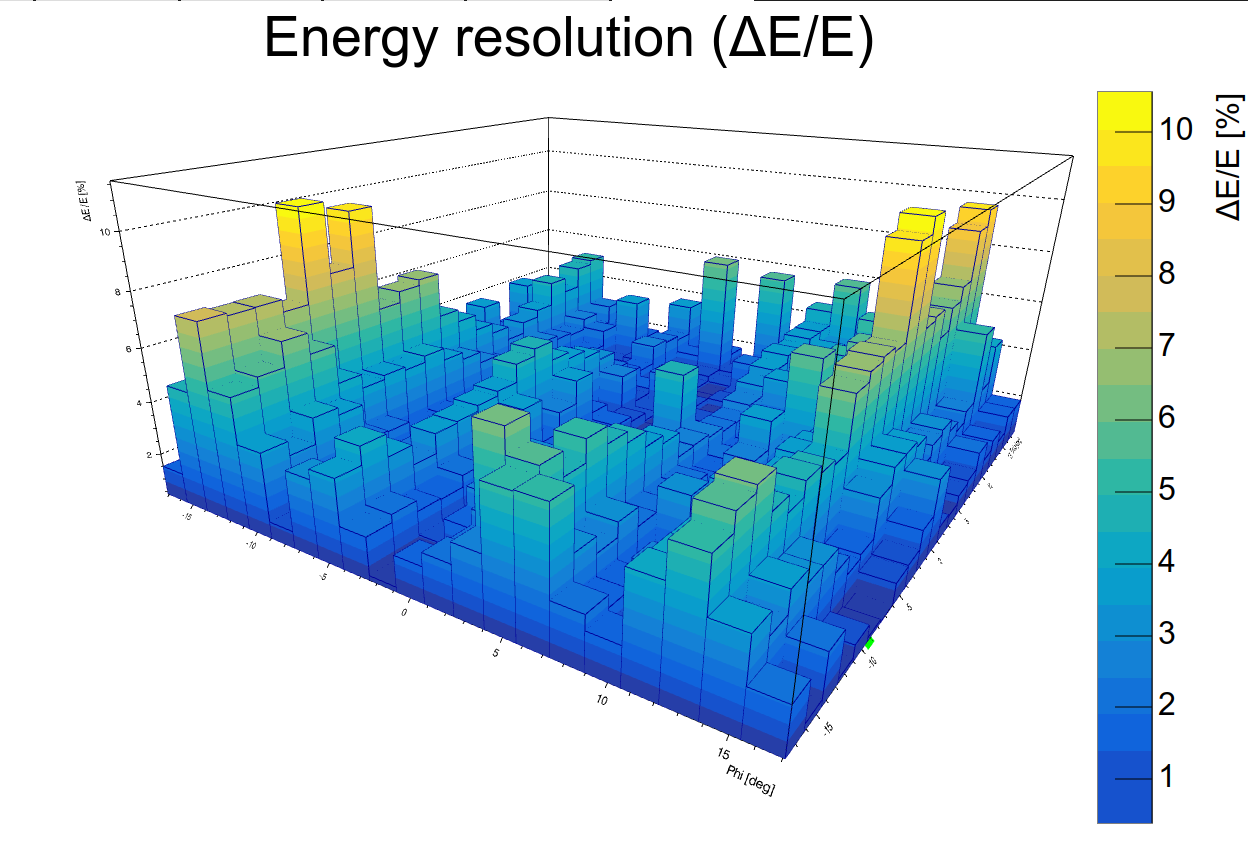
\includegraphics[width = 0.95 \linewidth]{images/c_p_theta_phi_abs.png}
				\end{figure}
			\end{columns}
		\end{frame}
		\begin{frame}
			\frametitle{Theta-Energy cut average error}
			\begin{columns}
				\column{0.5\textwidth}
				\centering
				\Large \textbf{Electrons}
				\begin{figure}
					\centering
					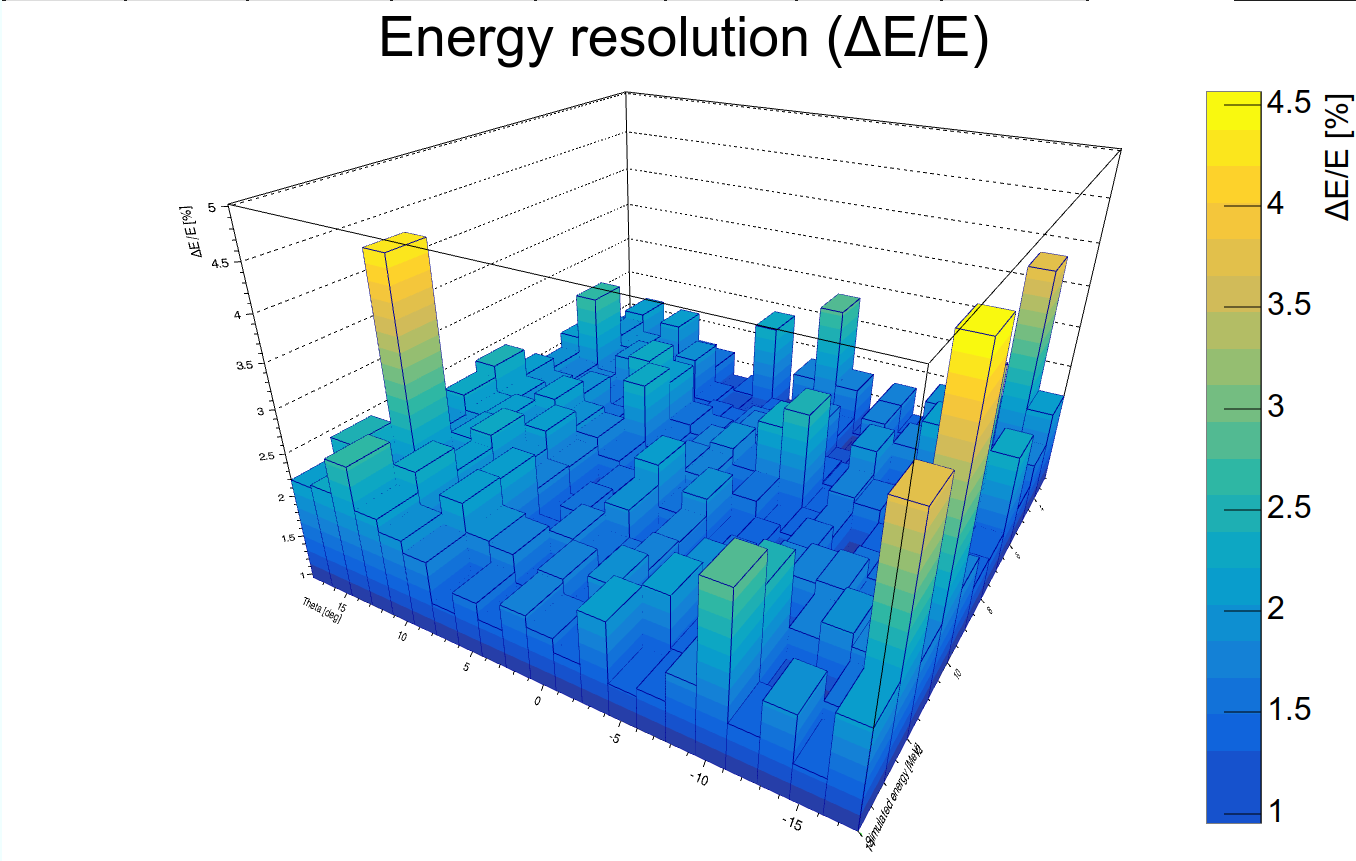
\includegraphics[width = 0.95 \linewidth]{images/c_e_theta_energy_abs.png}
				\end{figure}
				\column{0.5\textwidth}
				\centering
				\Large \textbf{Positrons}
				\begin{figure}
					\centering
					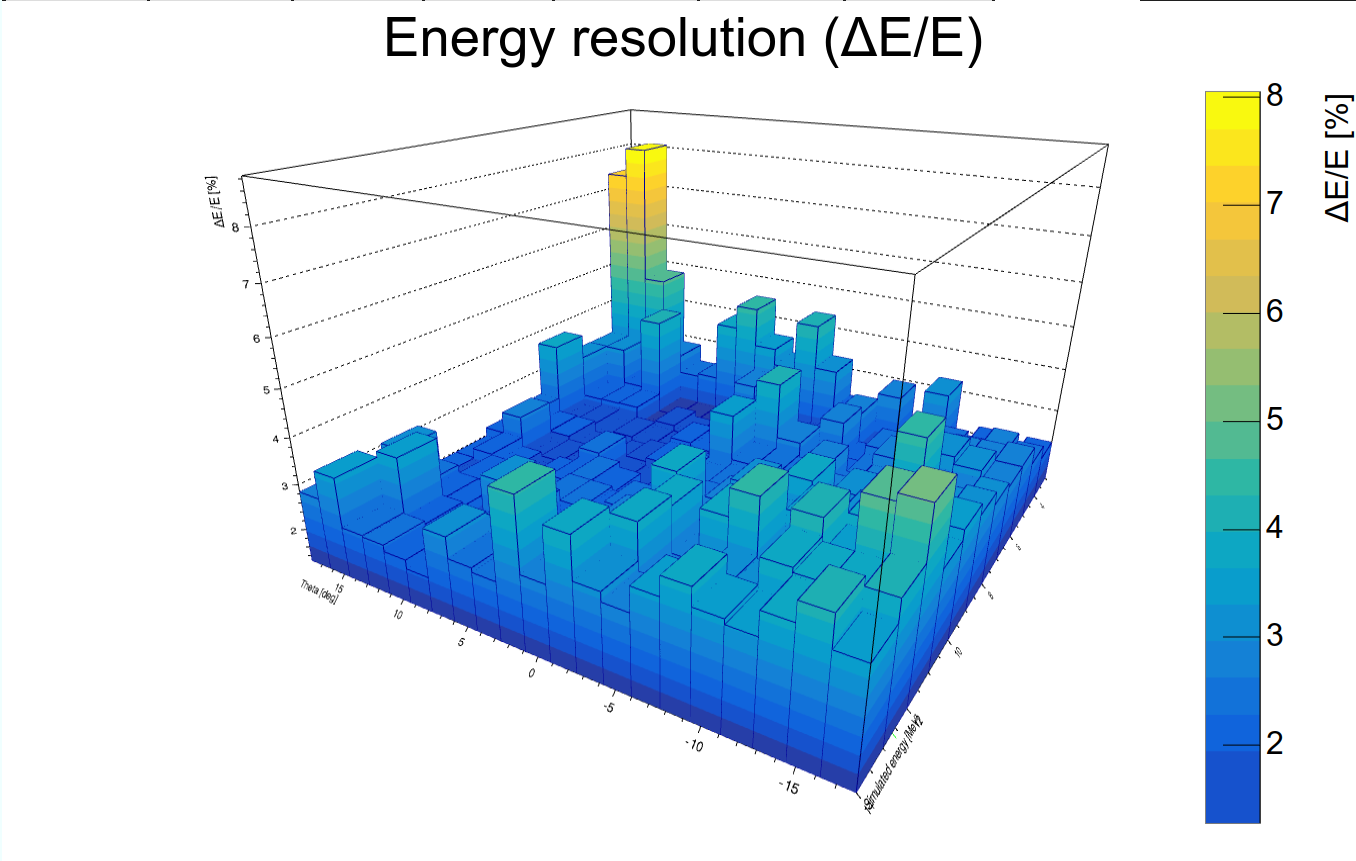
\includegraphics[width = 0.95 \linewidth]{images/c_p_theta_energy_abs.png}
				\end{figure}
			\end{columns}
		\end{frame}
		\begin{frame}
			\frametitle{Phi-Energy cut average error}
			\begin{columns}
				\column{0.5\textwidth}
				\centering
				\Large \textbf{Electrons}
				\begin{figure}
					\centering
					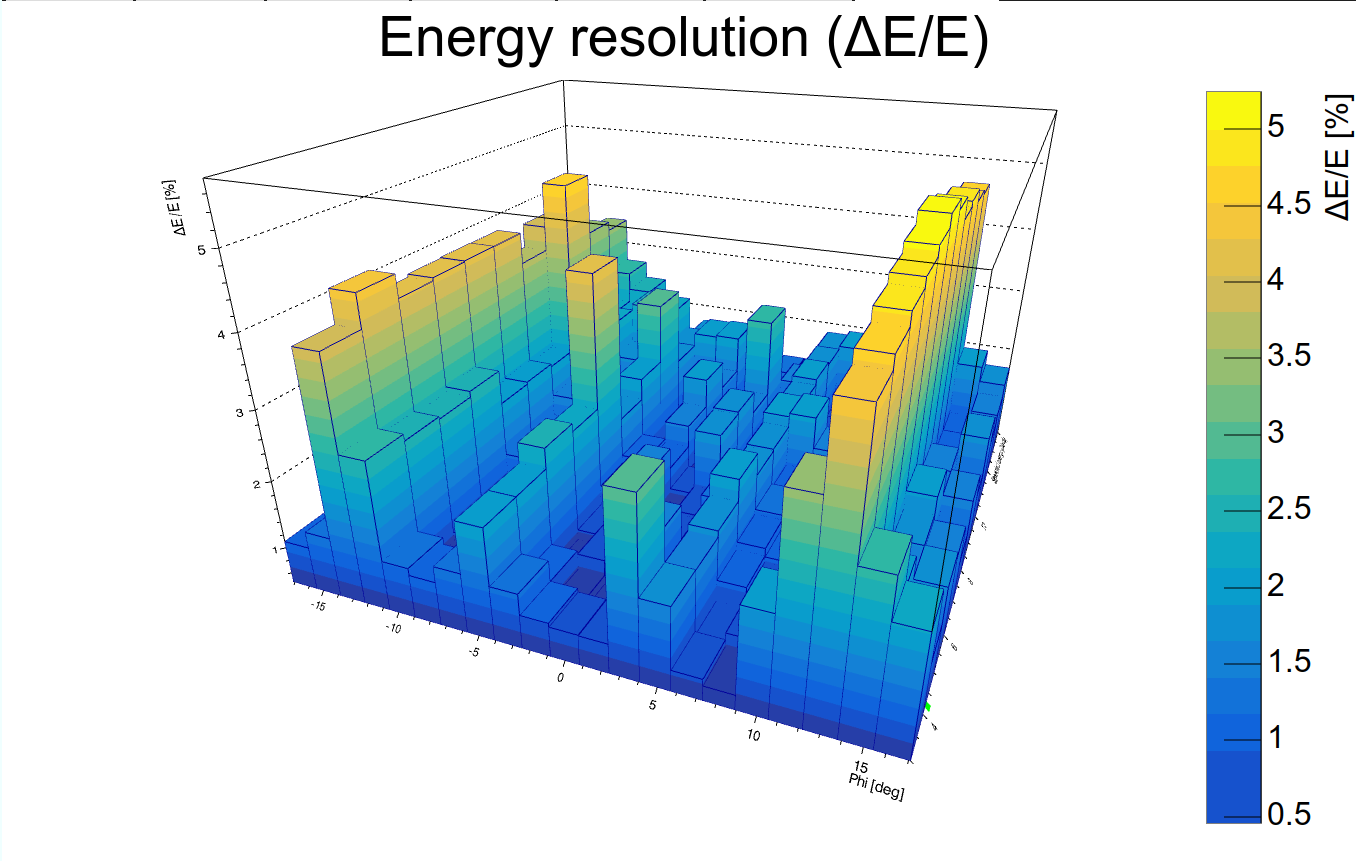
\includegraphics[width = 0.95 \linewidth]{images/c_e_phi_energy_abs.png}
				\end{figure}
				\column{0.5\textwidth}
				\centering
				\Large \textbf{Positrons}
				\begin{figure}
					\centering
					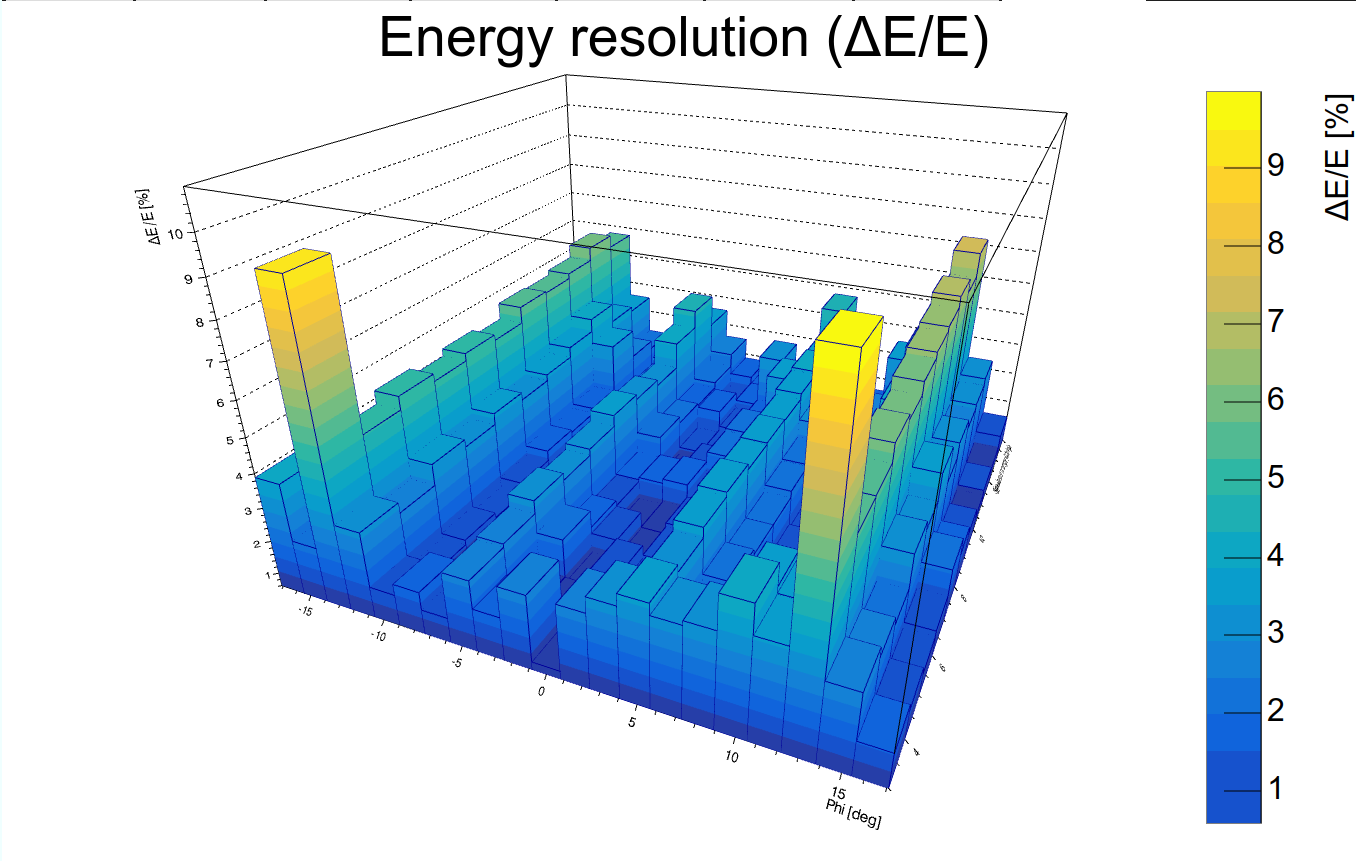
\includegraphics[width = 0.95 \linewidth]{images/c_p_phi_energy_abs.png}
				\end{figure}
			\end{columns}
		\end{frame}
	
	{
		%\usebackgroundtemplate{\includegraphics[width=\paperwidth,height=\paperheight]{images/DSC_5602.jpg}}%
		\begin{frame}[noframenumbering]{}
			\begin{center}
				\Huge Thank you for your attention.
			\end{center}
		\end{frame}
	}
	
	%\section{References}
	\begin{frame}[allowframebreaks,noframenumbering]
		\frametitle{References}
		%\printbibliography
		\bibliography{references}
		\bibliographystyle{unsrt}
	\end{frame}
	
\end{document}